\documentclass[sigconf, review, anonymous]{acmart}

\acmConference[WSDM '27]{ACM International Conference on Web Search and Data Mining}{February 2027}{Location TBD}
\acmYear{2027}
\acmISBN{}
\acmDOI{}
\setcopyright{none}

\usepackage{booktabs}
\usepackage{multirow}
\usepackage{amsmath,amssymb,amsthm}
\usepackage{xspace}
\usepackage{algorithm}
\usepackage{algorithmic}

%% Convenience macros
\newcommand{\method}{\textsc{Pewter}\xspace}
\newcommand{\ph}[1]{\textbf{[#1]}} % placeholder marker -- MUST BE EMPTY AT SUBMISSION
\newcommand{\Hh}{\mathrm{H}}
\newcommand{\MI}{\mathrm{I}}
\newcommand{\indeg}{\mathrm{in}}
\newcommand{\outdeg}{\mathrm{out}}

\theoremstyle{plain}
\newtheorem{proposition}{Proposition}
\newtheorem{lemma}{Lemma}
\newtheorem{corollary}{Corollary}
\theoremstyle{definition}
\newtheorem{definition}{Definition}
\newtheorem{assumption}{Assumption}
\newtheorem{remark}{Remark}

\begin{document}

\title{PEWTER: Predicting Edge Signs with Proximal Edge-Walk Transformers}

\author{Anonymous Author(s)}
\affiliation{%
  \institution{Anonymous Institution}
  \country{Anonymous Country}
}
\email{anon@email.com}

\begin{abstract}
Signed networks on the web, such as trust ratings on marketplaces, reviewer endorsements, and adminship votes, carry their label on edges rather than on vertices. The dominant approach for predicting such labels is vertex-centric: a graph neural network (GNN) embeds the two endpoints and maps the pair of embeddings to an edge label. We show that this design has an inherent limit. Because a message-passing GNN can only distinguish vertices up to their Weisfeiler-Leman (WL) colors, every edge sharing a WL color pair receives the same prediction, and the error is bounded below by the label entropy that survives that coarsening.  Empirically, baseline GNN accuracy on six public signed networks falls toward chance as this entropy rises. Edge sign is correlated over a short range - the mutual information between an edge sign and a neighboring edge sign drops by two to nearly five orders of magnitude between one and two hops in the line graph, so the usable signal is concentrated in a small labeled neighborhood. Interestingly, the signal is not symmetric and depends on the graph family. We thus propose to condition on both the labeled edges and the neighboring vertices near the target edge, instead of on only the two vertex summaries. We propose Pewter, which samples short walks that pass through the target edge, classifies the masked target sign with a transformer that reads each walk as a token sequence of both vertices and edges, and combines the walks containing an edge by a confidence-weighted vote. Pewter significantly improves test AUC over the strongest baseline per dataset -- drawn from a pool of generic and signed-graph-specific message-passing GNNs -- on all six datasets (mean $+3.3$ AUC points over the best baseline per dataset, range $+1.4$ to $+4.5$), with the largest gains on edges whose endpoints carry high label entropy, which is where the bound predicts vertex-centric models are weakest (up to $+0.26$ AUC on Bitcoin-otc and $+0.11$ on Epinions in the highest joint-entropy bins). Two interesting empirical observation are an asymmetry in the information flow of the edges and that in some graphs, most of the prediction is from edges and in others from vertices. We propose alternative theories for these differences. 
\end{abstract}

%% ACM Computing Classification System (CCS) Concepts
\begin{CCSXML}
<ccs2012>
   <concept>
       <concept_id>10010147.10010257.10010293.10010294</concept_id>
       <concept_desc>Computing methodologies~Neural networks</concept_desc>
       <concept_significance>500</concept_significance>
       </concept>
   <concept>
       <concept_id>10002951.10003260.10003282</concept_id>
       <concept_desc>Information systems~Web applications</concept_desc>
       <concept_significance>300</concept_significance>
       </concept>
 </ccs2012>
\end{CCSXML}

\ccsdesc[500]{Computing methodologies~Neural networks}
\ccsdesc[300]{Information systems~Web applications}

\keywords{Signed Graphs, Edge Sign Prediction, Graph Neural Networks, Random Walk Transformers, Trust and Reputation}

\maketitle

\section{Introduction}

Multiple web-based graphs put the label on the edge, not on the vertex. A buyer rates a seller as trustworthy or not on a peer-to-peer marketplace, a reviewer marks another reviewer as trusted or distrusted on a product review site, and an editor supports or opposes a candidate in an adminship election. In each case a directed edge carries a sign, most edges are unlabeled or unobserved, and the practical task is to predict the missing signs from the observed ones. 

The classical recipe for edge sign prediction extracts a fixed set of features around an edge, either external or topological, and classifies the edge from the vertex features (implicit or explicit)~\citep{leskovec2010predicting}. Such features were tradiionally hand-built and cannot adapt to the data. To address this, vertex-centric graph neural networks (GNNs)~\citep{kipf2016semi,gilmer2017neural} were proposed: Such GNNs produce an embedding for each vertex, and classify an edge from the pair of embeddings at its endpoints, optionally with some edge topological features~\citep{battaglia2018relational}. GNNs can reach a high accuracy when the endpoints determine the edge label. This accuracy degrades in a way that is predictable once we look at what a vertex embedding can and cannot hold.

Specifically, if a vertex is surrounded by edges of several classes, a single embedding cannot reproduce the different classes. The severity of the edge classificaiton limitation is controlled by the label entropy of the edges around that vertex, $\Hh(Y\mid v)$ (Section~\ref{sec:notation}). In practice, each edge is surrounded by both a source and target vertex, and the edge class is predicted by the embedding of both. However, even this is limited by the WL coloring~\citep{weisfeiler1968reduction} of the two surounding edges.  In a simple graph, each edge is fully defined by the vertices surrounding it. For an edge with an unknown class, a pair of vertices with the same WL coloring will always induce the same edge class.  We state this as Proposition~\ref{prop:bottleneck} and, in a capacity form, as Proposition~\ref{prop:capacity}, where we basically claim that vertex centric models are inherently limited. 

Instead, we propose a combined vertex and edge-centric approach based on the embedding of both edges and vertices and the classification through a random walk on edges. A limitation of random walk may be the high cost of performing long random walks along the graphs. However, we show that the mutual information between an edge's sign and a neighboring edge's sign collapses by two to nearly five orders of magnitude between line-graph distance 1 and distance 2--3 across all six datasets we study (Section~\ref{sec:empconf}). As such, almost all of the decodable signal about an edge sign sits in the labeled edges one hop away. We thus propose very short walks, which keeps the cost low, and show that such short walks are enough to drastically increase the edge classification accuracy.

%In directed graphs, an edge label need not be equally predictable from its two endpoints.  On four of the six datasets the label entropy seen from the source side is significantly lower than from the target side, so the source carries more of the label information; on the two Wikipedia vote graphs the direction significantly reverses. To ensure generality of Pewter, we perform walks starting two edges before the current edge and ending two edges after it, to allow a transformer the choice where to extract the information.  We call this directed short-path classifier Pewter (Proximal Edge-Walk Transformer with Ensemble Read-out).

\paragraph{Contributions.}
\begin{itemize}
\item We state and prove a limitation of vertex-centric edge classification: an information bottleneck controlled by the vertex label entropy that survives WL coarsening (Proposition~\ref{prop:bottleneck}), with an embedding-capacity form (Proposition~\ref{prop:capacity}). Unlike oversquashing, this bound is a property of the read-out and is not removed by rewiring, depth, or width.
\item We confirm the bottleneck empirically on six public signed networks, showing that the accuracy of edge-signed GNN baselines degrades on the high-entropy endpoints the bound points to (Figure~\ref{fig:empconf-panels}), and we quantify how fast edge-sign information decays with line-graph distance.
\item We report an asymmetry in edge class information of edges from/ to source and target vertices. This asymmetry varies across datasets. 
\item We propose Pewter, and show that it (1) improves AUC over eight baselines on all six datasets, and (2) improves accuracy most on edges whose endpoints have high label entropy, where the bound says vertex-centric models are weakest.
\item XXXXX  THE STRANGE DISTANT CORRELATIONS RESULTS TO BE REMOVED IF WE FIND MOTHING XXXXXX
\end{itemize}

\section{Related Work}
\paragraph{Edge and sign prediction.} Early work on signed network models predicted edge labels using local graph structure around an edge rather than its endpoints in isolation. Structural balance theory predicts a sign from the parity of a closed triad~\citep{cartwright1956structural}, and later work replaces balance with status differences and other triad-count features~\citep{leskovec2010predicting}. These methods rely on a fixed, hand-crafted set of local structural patterns rather than representations learned from data~\citep{naaman2019edge}. Pewter keeps the local, edge-centric view of this line of work and replaces the hand-built patterns with a learned sequence model.

\paragraph{Vertex-centric GNNs.}
\label{par:vertex-centric-gnns}
The dominant modern approach replaces hand-built triad features with message-passing GNNs specialized to signed and directed graphs~\citep{derr2018signed, huang2019signed, li2020learning, liu2021signed}. These architectures route positive and negative edges through separate aggregation pathways over one or more rounds of message passing, so that a vertex's representation is shaped differently by its friendly and hostile neighbors (positive or negative edges) rather than by a single undifferentiated aggregate, with some variants additionally aggregating in- and out-edges separately to track orientation. Edge signs are then predicted from the resulting pair of endpoint embeddings, optionally concatenated with edge features. Propositions~\ref{prop:bottleneck} and~\ref{prop:capacity} apply to every member of this family, since they constrain the read-out rather than the aggregation.

\paragraph{Walk and sequence representations.} A separate line of work embeds vertices from random walks over the graph~\citep{perozzi2014deepwalk, grover2016node2vec}, including signed-graph extensions of the same idea~\citep{kim2018side, islam2018signet}. There, the walk generates the training pairs, or context windows, used to fit a per-vertex embedding, and a downstream edge classifier reads a pair of such vertex embeddings, so the vertex bottleneck is reintroduced at the read-out. Sequence models applied directly to walks for vertex or graph classification process the walk token-by-token, but typically summarize it into one fixed per-vertex or per-graph vector before classification. Pewter differs in that the walk is never summarized into a vertex representation: the prediction is read at the masked edge position itself.

\paragraph{Graph transformers.} Transformer architectures~\citep{vaswani2017attention} have been adapted to attend over an entire graph or large subgraphs, using structural or positional encodings in place of a fixed adjacency prior~\citep{dwivedi2020generalization, ying2021transformers, rampavsek2022recipe}. Attention allows information to move between distant vertices in a single step rather than only through a fixed number of message-passing hops. These models typically attend over a vertex set and pool the result back down to one representation per vertex before an edge is scored, so they too are covered by Proposition~\ref{prop:bottleneck} whenever the final read-out is a function of two per-vertex vectors. Pewter attends over a short token sequence of alternating vertices and signed edges, which keeps attention cost independent of graph size.

\paragraph{Oversquashing and information bottlenecks.} A related line of work studies how message-passing GNNs lose information as receptive fields grow with depth: each vertex's neighborhood grows exponentially with the number of rounds while the message vector stays a fixed width, so distant information is compressed into a channel too narrow to carry it~\citep{alon2020bottleneck, topping2021understanding}. That bottleneck is a property of propagation depth and can in principle be mitigated by rewiring. The bottleneck of Propositions~\ref{prop:bottleneck} and~\ref{prop:capacity} is different in kind: it is a property of the read-out step, and applies to a single fixed-width vertex embedding regardless of how many rounds produced it or how the graph was rewired.

\section{Problem Setting and Notation}
\label{sec:notation}
Let $G=(V,E)$ be a graph, directed unless stated otherwise, and let each edge $e\in E$ carry a label $y_e$ from a finite set $\mathcal{C}$ of size $|\mathcal{C}|=c$ (for sign prediction, $c=2$; the propositions hold for general $c$). We observe labels on $E_{\mathrm{obs}}\subset E$ and predict $y_e$ for $e\in E\setminus E_{\mathrm{obs}}$.

\label{def:vertex-entropy}For a vertex $v$ we write $\Hh(Y\mid v)$ for the entropy of the label distribution over the edges incident to $v$, split into $\Hh_\indeg(v)$ over in-edges and $\Hh_\outdeg(v)$ over out-edges. For an edge $e$ we write $\Hh_{\mathrm{src}}(e)=\Hh_\outdeg(u)$ for the out-edge entropy at its source $u$ and $\Hh_{\mathrm{tgt}}(e)=\Hh_\indeg(v)$ for the in-edge entropy at its target $v$. For a random variable $Z$ we write $\Hh(Y\mid Z)$ for conditional entropy and $\MI(Y;Z)$ for mutual information. We use Fano's inequality~\citep{cover2006elements}: for any predictor $\hat Y=g(Z)$ of $Y$ over $c$ classes with error probability $P_e$ and entropy $\Hh_b(P_e)$,
\begin{equation}
\Hh(Y\mid Z)\le \Hh_b(P_e)+P_e\log(c-1).
\label{eq:fano}
\end{equation}

Our empirical setting is binary sign prediction, $c=2$, where $\log(c-1)=0$ and \eqref{eq:fano} holds with no weakening: $\Hh(Y\mid Z)\le \Hh_b(P_e)$. Since $\Hh_b$ is a strictly increasing bijection $[0,\tfrac12]\to[0,1]$ its inverse $\Hh_b^{-1}$ is strictly increasing (Appendix~\ref{app:proofs}, Lemma), and any predictor with $P_e>\tfrac12$ can be improved by flipping its output, so the bound inverts to
\begin{equation}
P_e\ \ge\ \Hh_b^{-1}\big(\Hh(Y\mid Z)\big).
\label{eq:invfano}
\end{equation}
This is the form we use throughout: larger conditional entropy of the conditioning variable forces larger error, for every model. We set $\Hh_b^{-1}(x):=0$ for $x\le 0$ by convention, so \eqref{eq:invfano} stays well defined, and trivially true rather than undefined, when its argument is non-positive. For clarity, we use sign instead of (the binary) label along the following text, except in formal notation and the compound term "label entropy," which we use interchangeably with "sign"/"sign entropy" throughout.

We use \eqref{eq:invfano} rather than the more familiar linear corollary $P_e\ge\frac{\Hh(Y\mid Z)-1}{\log c}$ because at $c=2$ the latter is vacuous: $\log c=1$ and $\Hh(Y\mid Z)\le 1$ bit, so its right-hand side is never positive. 
%The linear form remains valid and useful for $c>2$ and is restated in Appendix~\ref{app:proofs}, together with an explicit Pinsker-type relaxation of \eqref{eq:invfano} XXX REF XXX for readers who prefer a closed form to an inverse function.
\section{Limitations of Vertex-Centric Edge Classification}
A vertex-centric edge classifier is any map $\hat y_{uv}=g(h_u,h_v)$, where $h_u=\phi(\mathcal{T}_u)$ is a vertex representation computed from the rooted computation tree $\mathcal{T}_u$ of $u$, and $g$ is arbitrary. This covers GCN~\citep{kipf2016semi}, GraphSAGE~\citep{hamilton2017inductive}, GAT~\citep{velivckovic2017graph}, and the signed GNNs of Section~\ref{par:vertex-centric-gnns} with an edge read-out. Let $\chi(\cdot)$ denote the stable WL coloring~\citep{weisfeiler1968reduction}. Any message-passing GNN factors through it~\citep{xu2018powerful, morris2019weisfeiler}, so $h_u=\psi(\chi(u))$ for some $\psi$ and $\hat y_{uv}=\tilde g(\chi(u),\chi(v))$.

\begin{assumption}[Structural regime]
\label{as:structural}
The endpoints enter the read-out only through their WL colors $\chi(u),\chi(v)$, and these colors are not injective on the edges we predict: with positive, and in practice non-negligible, probability, a WL color pair $(\chi(u),\chi(v))$ is shared by two edges of different sign.
\end{assumption}

This assumption is forced whenever the endpoints of test edges are unseen at training time, and it holds inside any graph with structural symmetry or repeated motifs. Note that in theory, a model that learns a free embedding per vertex, indexed by identity, escapes the WL coarsening and therefore escapes Proposition~\ref{prop:bottleneck}, at the price of not transferring to new vertices and of fitting one parameter vector per vertex. 

\begin{proposition}[Endpoint bottleneck]
\label{prop:bottleneck}
Under Assumption~\ref{as:structural}, every vertex-centric edge classifier $\hat y_{uv}=g(h_u,h_v)$ has population error
\[
P_e \ \ge\ \Hh_b^{-1}\Big(\Hh\big(Y\mid \chi(U),\chi(V)\big)\Big)\ >\ 0,
\]
for a random edge $(U,V)$. The quantity $\Hh(Y\mid \chi(U),\chi(V))$ is the label entropy that remains after endpoint identities are replaced by their WL colors, and it does not decrease with depth or width.
\end{proposition}

\begin{proof}[Proof sketch]
Any message-passing GNN factors as $\tilde g(\chi(U),\chi(V))$, so it is measurable with respect to the color pair. Among such predictors the error is minimized by the majority label in each color class; applying \eqref{eq:invfano} within each color pair and combining across pairs via Jensen's inequality, using convexity of $\Hh_b^{-1}$ 

XXX NEED TO CHECK CAREFUllY XXXX

(Appendix~\ref{app:proofs}), gives the bound. Assumption~\ref{as:structural} makes the entropy positive, hence $P_e>0$. Full argument, including the general-$c$ form, in Appendix~\ref{app:proofs}.
\end{proof}

\begin{remark}
As noted above, in a simple graph the two vertex \emph{identities} fix the single edge between them, so $\Hh(Y\mid U,V)=0$. This is not the quantity that bounds a structural GNN. Message passing cannot see past the WL colors, and identities neither survive that coarsening nor transfer to a held-out edge whose endpoints were never seen carrying that label. The bottleneck is set by the resolution of the representation, not by whether the graph carries more than one edge per pair.
\end{remark}

\begin{corollary}[Single-endpoint reading]
\label{cor:endpoint}
Fix a source $u$ and a target color $b$. Every edge from $u$ to a target of color $b$ receives one prediction, so the error on that group is at least $\Hh_b^{-1}\big(\Hh(Y\mid \text{source}{=}u,\ \text{target color}{=}b)\big)$. A source whose out-edge labels are mixed and are not separated by target color, that is, high $\Hh_\outdeg(u)$ left unresolved by $\chi(V)$, forces error on those edges for every such model.
\end{corollary}

Informally, high endpoint entropy breaks the vertex-centric read-out. The same claim can be made from the side of the embedding width rather than the coloring.

\begin{proposition}[Capacity form]
\label{prop:capacity}
Suppose each vertex representation takes at most $N$ distinguishable values under the read-out (for width $d$ at $b$ bits per coordinate, $N=2^{bd}$; in general $N$ is the covering number of the representation space at the decision margin of $g$). Then
\[
\MI\big(Y;h_U,h_V\big)\ \le\ 2\log N,
\qquad
P_e\ \ge\ \Hh_b^{-1}\big(\Hh(Y)-2\log N\big).
\]
Per vertex, $h_U$ carries at most $\log N$ bits about the joint label of all edges at $U$, so if $U$ has out-degree $D$ with near-independent out-edge labels of entropy $\Hh_\outdeg(U)$ each, then $D\,\Hh_\outdeg(U)-\log N$ bits are unrecoverable once $D\,\Hh_\outdeg(U)>\log N$.
\end{proposition}

\begin{proof}[Proof sketch]
$\MI(Y;h_U,h_V)\le \Hh(h_U)+\Hh(h_V)\le 2\log N$ since each embedding takes $\le N$ values; substitute into $\Hh(Y\mid h_U,h_V)=\Hh(Y)-\MI(Y;h_U,h_V)$ and apply \eqref{eq:invfano} with the monotonicity of $\Hh_b^{-1}$. The per-vertex statement is the same cardinality bound on $h_U$ alone. XXXX AGAIN CHEKC XXXXX Details in Appendix~\ref{app:proofs}.
\end{proof}
The two statements say the same thing from two sides. Depth and width do not help, because the object being conditioned on, the endpoint summary, is the bottleneck. 

\section{Methods}
\label{sec:methods}
Pewter has three parts: a random-walk sampler over the signed graph, a per-walk transformer that classifies a masked target edge from its surrounding walk context, and a validation-tuned weighted vote across the scores of the same edge across walks. Figure~\ref{fig:pipeline-schematic} sketches the pipeline.

\begin{figure*}[t!]
\centering
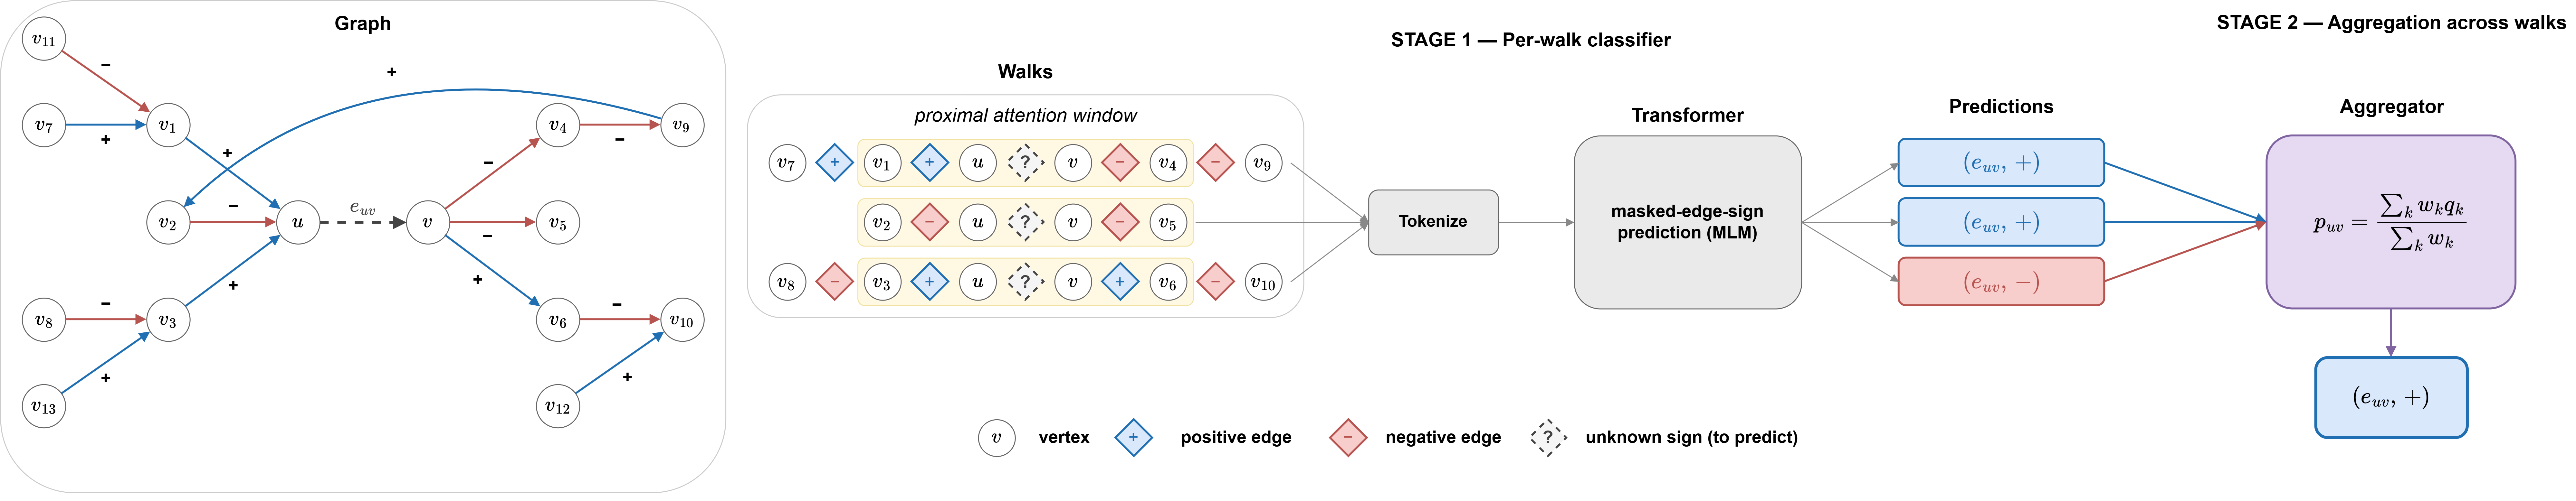
\includegraphics[width=\linewidth]{figures/pipeline_schematic.png}
\caption{\method\ trains two separate models for one target edge $(u,v)$. \textbf{Stage 1} (left): walks through $(u,v)$ are sampled, sign-masked (`?'), tokenized, and scored by a frozen Transformer within a $\pm2$-hop window; the three example walks disagree, giving predictions $q_1,q_2$ (positive) and $q_3$ (negative). \textbf{Stage 2} (right, purple): an aggregator combines the $k$ per-walk predictions into one score, $p_{uv}=\sum_k w_k q_k/\sum_k w_k$. Legend: V = vertex, `+'/`-' = edge sign, `?' = the masked target edge. XXX Need larger fonts in the plot XXXXXXX}
\label{fig:pipeline-schematic}
\end{figure*}

\paragraph{Walk sampler.} We build the walk corpus in two passes. First, every edge gets one walk that starts by traversing it: from its source vertex, cross that edge, then continue as an ordinary random walk for the remaining hops. This alone guarantees that every edge is covered by at least one walk. Second, we fill the rest of the $M$-walk budget with additional walks: each one first finds a short directed path leading into a random vertex, then continues forward from that vertex for the remaining hops, and is checked with a hash against every walk already in the corpus; if it repeats one already collected, we discard it and draw another, so that no two of the $M$ walks coincide. Traversal is directed. Each walk is encoded as an alternating sequence of vertex and edge tokens $N_{u_0}, E_{s_1}, N_{u_1}, E_{s_2}, \ldots$, where $E_{s_i}\in\{+1,-1\}$ is the observed sign of the traversed edge. Because each walk touches up to $L$ edges, a given edge typically appears as a token inside many walks, not just the one it anchors; these occurrences are combined by the vote below.

\paragraph{Per-walk classifier.} Each walk is embedded token-by-token through a single shared embedding table (vertices, edge signs, and special tokens all share one vocabulary, dimension $d$), given fixed sinusoidal positional encodings, and passed through a Transformer encoder~\citep{vaswani2017attention} ($n_\text{layer}$ layers, $n_\text{head}$ heads). We consider two self-attention variants: \emph{full} attention, where every token attends to every other token in the walk, and \emph{local} attention, where token $i$ attends only to tokens $j$ with $|i-j|\le w$; since each graph hop spans two token positions, $w=4$ restricts every token to roughly its $\pm2$-hop surroundings (see Figure~\ref{fig:empconf-panels}(A) for the position-index notation). At each epoch, a fresh $40\%$ of the currently-visible edges is resampled as that epoch's prediction targets, stratified to preserve the positive/negative class balance. Each designated edge has its sign token hidden but remains fully attendable as context for other predictions -- a stricter, split-based exclusion is described next. The model predicts a hidden position's sign from its surrounding vertex and edge context through a shared linear classification head, in the style of masked language modeling~\citep{devlin2019bert}. The model is trained end-to-end with a cross-entropy loss over the two sign classes, computed only at the hidden target positions; every other position, hidden or not, contributes no loss. A second regularizer randomly replaces a fraction $p$ of vertex-identity tokens with an unknown-vertex placeholder or another vertex's token, so the model cannot fall back on memorized vertex identity in place of structural and sign context.

\paragraph{No label leakage.} The walk corpus is built once from the full graph, independent of any split, so a sampled walk can pass through an edge whose split is not yet meant to be visible: a validation or test edge can appear while training, and a test edge can appear while validating. Every occurrence of such an edge, in every walk that happens to contain it, has its sign token replaced by \texttt{<MASK>} and is additionally excluded from attention as a key, not just hidden as a target -- so it cannot inform the prediction of any edge, including its own. This is stricter than the target masking described above: a masked prediction target keeps its position attendable, with only its sign hidden, whereas a split-excluded edge is invisible altogether.

\paragraph{Aggregation across walks.} A given edge occurs in many sampled walks, each yielding a probability estimate $q_j=P(\text{sign}=1\mid \text{walk}_j)$. We combine these into an edge-level score with a parametric weighted mean, $\hat{y}_e = \frac{\sum_j w_j q_j}{\sum_j w_j}$, with weights $w_j = |\operatorname{logit}(q_j)|^{b}$, where $b$ is fit by maximizing validation AUC~\citep{nelder1965simplex}. The weighting has a natural reading: $|\operatorname{logit}(q_j)|$ is a monotone decreasing function of the walk-level predictive entropy, so the aggregator symmetrically up-weights confident walk occurrences over uncertain ones, regardless of which class they favor. This is a standard confidence-weighted ensemble rule, comparable to inverse-variance weighting, rather than a fitted heuristic; Ablation~B shows that the specific choice barely matters, so we present it as a defensible default rather than as a contribution. The per-walk estimates are not independent, since walks overlap, so the weighted mean should be read as a variance-reducing pooling rule and not as a likelihood. Algorithm~\ref{alg:pewter} gives the full inference procedure for one edge.

\begin{algorithm}[tb]
\caption{\method: inference for edge $(u,v)$}
\label{alg:pewter}
\textbf{Input}: target edge $(u,v)$; walk corpus; per-walk classifier $f_\theta$, already trained; aggregator weight function $w(\cdot)$\\
\textbf{Output}: predicted sign probability $\hat y_{uv}$
\begin{algorithmic}[1]
\STATE Let $W_1,\ldots,W_K$ be the $K$ corpus walks containing $(u,v)$
\FOR{$j = 1$ to $K$}
  \STATE Tokenize $W_j$ as alternating vertex/edge tokens, masking $(u,v)$'s sign
  \STATE $q_j \gets f_\theta(W_j)$ \COMMENT{per-walk class-1 probability}
\ENDFOR
\STATE $\hat y_{uv} \gets \frac{\sum_j w(q_j)\, q_j}{\sum_j w(q_j)}$
\STATE \textbf{return} $\hat y_{uv}$
\end{algorithmic}
\end{algorithm}

\paragraph{Datasets.} We evaluate on six public directed signed-graph benchmarks. \textsc{Bitcoin-alpha} (3{,}783 vertices, 24{,}186 edges) and \textsc{Bitcoin-otc} (5{,}881 vertices, 35{,}592 edges) are peer-to-peer marketplace trust networks~\citep{kumar2016edge, kumar2018rev2}: an edge $u\to v$ is a $-10$ to $+10$ trust rating (excluding $0$), of which we keep only the sign (positive/negative) and drop the magnitude. \textsc{Epinions} (131{,}580 vertices, 840{,}799 edges) and \textsc{Slashdot} (82{,}140 vertices, 549{,}202 edges) are review-site and news-site trust/friend networks~\citep{leskovec2010signed}, already binary (trust/distrust, friend/foe) in the source data. \textsc{Wiki-elec} (7{,}115 vertices, 103{,}689 edges) and \textsc{Wiki-RfA} (11{,}256 vertices, 177{,}211 edges) are Wikipedia adminship-election vote networks~\citep{leskovec2010signed, leskovec2010predicting, west2014exploiting}: an edge $u\to v$ is one voter's ballot on one candidacy, support ($+$) or oppose ($-$); both also allow a neutral ballot, a minority of all cast votes ($6.1\%$ on both) that we drop, keeping only support/oppose. Edge signs are heavily imbalanced toward positive/trust in all six (77--94\% positive).

Self-loops are removed everywhere ($573$ edges on Epinions, none on the other five). On Wiki-elec and Wiki-RfA, when the same voter casts more than one ballot on the same candidacy we keep only the most recent one, which collapses $3.1\%$ and $3.9\%$ of their non-neutral votes respectively; the other four datasets have no repeated directed pairs to begin with, so this does not affect them. Each graph is then split 80/10/10 into train/validation/test with a fixed seed; the training portion is further split into a context pool and a masking pool of fixed relative size ($48\%/32\%$ of the total); which edges within this combined pool serve as supervised targets is not fixed, but resampled every epoch (see the Per-walk classifier paragraph above).

\paragraph{Baselines.} We compare against two generic message-passing GNNs that ignore edge sign (GCN~\citep{kipf2016semi}, GAT~\citep{velivckovic2017graph}), four signed-graph-specific methods (SGCN~\citep{derr2018signed}, SiGAT~\citep{huang2019signed}, GS-GNN~\citep{liu2021signed}, SNEA~\citep{li2020learning}), and a recent correlation-modeling method (CopulaLSP~\citep{sung2026scalable}). We additionally compare against node2vec~\citep{grover2016node2vec}, a non-signed-aware walk embedding, as a non-GNN reference point.

\begin{table}[h!]
\centering
\scriptsize
\caption{Per-dataset size and walk budget. $\kappa$ is the walk-budget multiplier, $M=\kappa|E|$, fixed per dataset (Setup below).}
\label{tab:dataset-walks}
\begin{tabular}{lrrrr}
\toprule
Dataset & Vertices & Edges $|E|$ & $\kappa$ & Walks $M$ \\
\midrule
Bitcoin-alpha & 3{,}783 & 24{,}186 & $5$ & 120{,}930 \\
Bitcoin-otc & 5{,}881 & 35{,}592 & $5$ & 177{,}960 \\
Epinions & 131{,}580 & 840{,}799 & $1$ & 840{,}799 \\
Wiki-elec & 7{,}115 & 103{,}689 & $1.5$ & 155{,}534 \\
Wiki-RfA & 11{,}256 & 177{,}211 & $1.5$ & 265{,}817 \\
Slashdot & 82{,}140 & 549{,}202 & $3$ & 1{,}647{,}606 \\
\bottomrule
\end{tabular}
\end{table}

\paragraph{Setup.} \method's per-walk transformer architecture and optimizer are tuned per dataset rather than shared: across the six datasets, embedding dimension $d\in[32,128]$, $n_\text{head}\in[2,8]$, feed-forward dimension $\in[32,256]$, $n_\text{layer}\in[3,5]$, dropout $\in[0.001,0.20]$, and learning rate $\in[1\times10^{-4},3\times10^{-3}]$; batch size is fixed at 1024 for all six, and every run uses early stopping on validation AUC (up to 50--75 epochs depending on dataset). Exact per-dataset values are in the released configuration files rather than enumerated here. Walks have varying length up to a maximum $L=80$ hops; the local-attention window means that even a long walk contributes only a $\pm2$-hop context to each prediction, so the effective receptive field is short even though the sampled sequence need not be. The total walk budget $M$ is fixed per dataset, like the rest of the per-dataset configuration above (Table~\ref{tab:dataset-walks}).

\paragraph{Statistical evaluation and reproducibility.} We evaluate on 10 independent 80/10/10 train/validation/test splits (seeds 42--51) and report the mean $\pm$ std test AUC across them. The exact splits, the sampled walk corpora, and the configuration files for every number in this paper are released in an anonymized repository \ph{ANONYMOUS GITHUB LINK}; each individual run uses a single NVIDIA L40S GPU. 
We name the test behind every comparative claim rather than reporting point estimates alone. Paired AUC comparisons across the 10 splits (e.g.\ \method\ against the best baseline, or one bucket against another) use a one-sided paired Wilcoxon signed-rank test, which does not assume normally-distributed differences. Where a quantity is tested jointly against two factors, we use a two-way ANOVA with the 10 splits as repeated measurements. Per-vertex paired quantities are tested per dataset with the same paired Wilcoxon test, then pooled across datasets via a random-effects meta-analytic estimate~\citep{dersimonian1986meta}. Where many coefficients are fit independently per split, robustness is assessed with cluster-robust standard errors~\citep{cameron2011robust} and a Benjamini-Hochberg FDR correction~\citep{benjamini1995controlling} rather than any single split's significance. Directional asymmetries in per-edge or per-token quantities are tested with cluster-robust confidence intervals, clustered at the level of the repeated unit. XXX VERIFY REFS XXX

\section{Results}

\subsection{Empirical Confirmation of the Bottleneck}
\label{sec:empconf}
To test for the association between edge signs across edges and vertices,  we evaluate edge sign correlations and edge sign prediction accuracy on the six directed signed-graph datasets described in Section~\ref{sec:methods} (Datasets). The test AUC of the prediction is computed on message-passing and signed-GNN baselines listed there. Here and along the paper, we treat the edge of interest as position 0, the vertices surrounding it as positions -1 and 1, the following edges as positions -2 and 2 and so on (Figure~\ref{fig:empconf-panels}A)

\paragraph{(A) Information decays sharply with distance.}
Mutual information between an edge's sign and a nearby edge's sign collapses by two to nearly five orders of magnitude ($178\times$--$73{,}000\times$ across the six datasets) between line-graph distance 1 (edges sharing a vertex) and distance 2--3 (Figure~\ref{fig:empconf-panels}B). The decodable signal is concentrated within about one hop. Thus, one can limit the attention to short walks as detailed in section~\ref{sec:methods}.

\paragraph{(B) Baseline accuracy falls as endpoint entropy rises.}
Each vertex has four associated entropies, one per incident-edge direction and endpoint role: $\Hh_\outdeg(-1)$/$\Hh_\indeg(-1)$ for the source $u$'s own out-/in-edges, and $\Hh_\outdeg(1)$/$\Hh_\indeg(1)$ for the target $v$'s (Figure~\ref{fig:empconf-panels}A); each is the binary entropy of that edge set's sign distribution. For example, a vertex with 8 positive and 2 negative out-edges has $\Hh_\outdeg=\Hh_b(0.8)\approx0.72$, one with 5 of each has $\Hh_\outdeg=\Hh_b(0.5)=1$ (maximal disagreement), and one with unanimous out-edges has $\Hh_\outdeg=0$. Proposition~\ref{prop:bottleneck} gives the theoretical reason to expect AUC to fall as this entropy rises: the bound is driven by how mixed the true sign is among edges that collapse to the same WL color, and high incident-edge entropy at an endpoint is exactly where that mixing is severe, so an endpoint's own local label heterogeneity is a direct proxy for how tight its accuracy ceiling is. Baseline test AUC drops as a function of source-vertex entropy, as Proposition~\ref{prop:bottleneck} predicts: for SiGAT, on all six datasets, AUC is highest where the target vertex's incoming-edge signs are unanimous and falls toward chance as that entropy rises, with source out-entropy a secondary factor (Figure~\ref{fig:empconf-panels}C,E). A two-way ANOVA per dataset (source out-entropy bin $\times$ target in-entropy bin, treating the 10 splits as repeated measurements) finds both main effects significant on all six datasets ($p<0.01$); their interaction is significant on five of six, the exception being Bitcoin-alpha, whose smaller test set leaves several bins underpowered.

\paragraph{(C) Entropy asymmetry is significant within datasets and heterogeneous across them.}
A per-vertex paired test of $\Hh_\outdeg(v)$ against $\Hh_\indeg(v)$ across all six datasets shows that on four (Bitcoin-alpha, Bitcoin-otc, Epinions, Slashdot) source-side entropy is lower with overwhelming per-dataset significance ($p$ from $5.1\times10^{-4}$ to $3.7\times10^{-244}$, one-sided Wilcoxon signed-rank test), while on two (Wiki-elec, Wiki-RfA) the direction reverses, itself significantly ($p=1.7\times10^{-10}$ and $3.4\times10^{-14}$). A pooled random-effects estimate across the four confirming datasets gives $58.1\%$ of non-tied vertex pairs favoring lower source entropy (95\% CI $[55.3\%, 60.8\%]$); pooled across all six the estimate is not significant, its interval spanning the null. 
\paragraph{(D) Different .}
A per-vertex paired test of $\Hh_\outdeg(v)$ against $\Hh_\indeg(v)$ across all six datasets shows that on four (Bitcoin-alpha, Bitcoin-otc, Epinions, Slashdot) source-side entropy is lower with overwhelming per-dataset significance ($p$ from $5.1\times10^{-4}$ to $3.7\times10^{-244}$, one-sided Wilcoxon signed-rank test), while on two (Wiki-elec, Wiki-RfA) the direction reverses, itself significantly ($p=1.7\times10^{-10}$ and $3.4\times10^{-14}$). A pooled random-effects estimate across the four confirming datasets gives $58.1\%$ of non-tied vertex pairs favoring lower source entropy (95\% CI $[55.3\%, 60.8\%]$); pooled across all six the estimate is not significant, its interval spanning the null. 

\begin{figure}[t!]
\centering
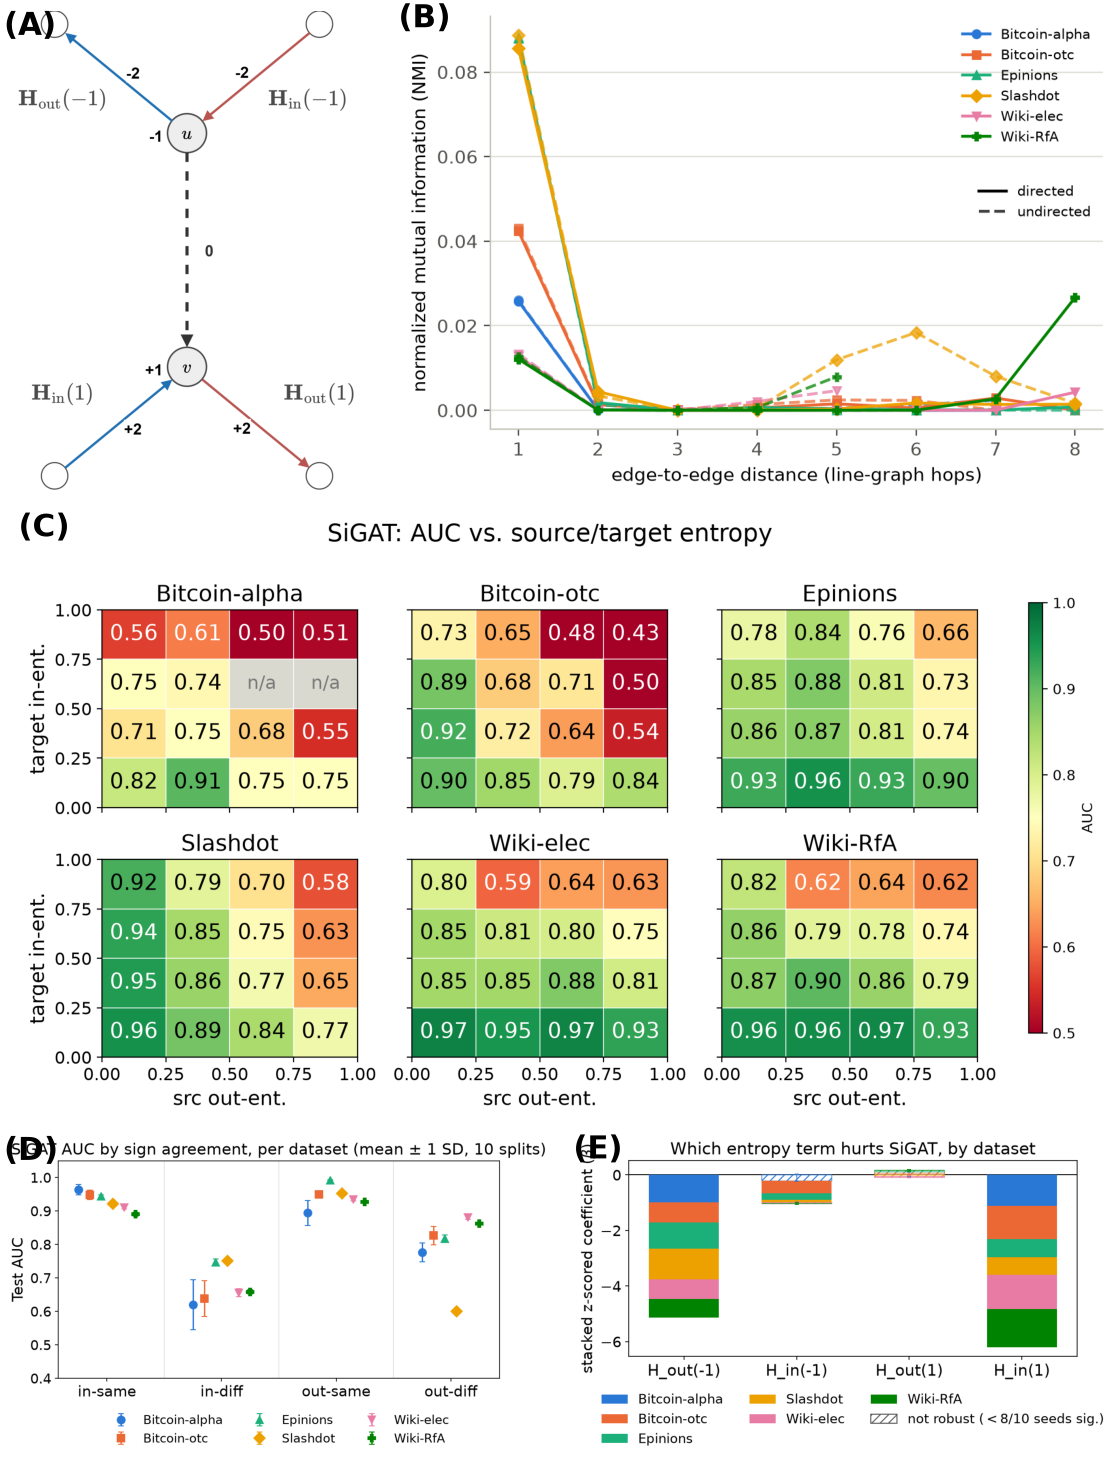
\includegraphics[width=\linewidth]{figures/empconf_panels_abcde_combined_sidebyside.png}
\caption{\footnotesize (A) Position-index notation used throughout: target edge = index 0, source $u$ = $-1$, target $v$ = $+1$; each endpoint's other incident edges are indexed $\pm2$, split into out-edges ($\Hh_\outdeg$) and in-edges ($\Hh_\indeg$). (B) Normalized mutual information ($\mathrm{NMI}=\MI/\Hh(Y)$, comparable across datasets with different label imbalance) between an anchor edge's sign and a context edge's sign vs. line-graph distance (1 = share a vertex), six datasets; solid = directed traversal, dashed = undirected (used throughout the rest of the paper). (C) Test AUC (discrete $4\times4$ bins) for SiGAT vs. source out-entropy ($\Hh_\outdeg(-1)$, rater consistency) and target in-entropy ($\Hh_\indeg(1)$, reputation contestedness), six datasets. (D) Test AUC (mean $\pm1$ SD, 10 splits) for SiGAT, one dot per dataset, bucketed by whether a target edge's other in-edges (into $v$) or out-edges (from $u$) agree (\emph{same}) or disagree (\emph{diff}) with it; an edge can appear in multiple buckets since each qualifying neighbor edge contributes one instance. A paired Wilcoxon test (10 splits) confirms AUC is higher for \emph{same} than \emph{diff} on both axes, all six datasets ($p=0.001$ throughout). (E) $z$-scored logistic-regression coefficients (correct $\sim \Hh_\outdeg(-1)+\Hh_\indeg(-1)+\Hh_\outdeg(1)+\Hh_\indeg(1)$) for SiGAT, refit per dataset on 10 splits; each term's bar is stacked by dataset (diverging: negative segments stack downward) to compare across datasets rather than only pooled; error bars are $\pm1$ SD per segment, hatched = not robust (BH-FDR significant in $<8/10$ seeds).}
\label{fig:empconf-panels}
\end{figure}

\subsection{Pewter is more accurate than SOTA}
XXXX THIS IS THE FIRST TIME PEWTER IS DECRIBED SO NEED A SHORT EXPLANATION HERE OF WHAT PEWTER DOES WITH AT LEAST 4 OR 5 SENTENCES (WITH REFERENCE TO FIGURE 1) AND THEN AN EXPLANATION OF ALL THE BASELINES WE COMPARE AND  AS DESCRIPTION OF THE RESULTS OF TABLE 1, INCLUDING A STATISTICAL TEST, THEN DESCRIBE FIGURE 3 AND ADD THERE A STATISITCAL CLAIM ON THE DIFFERENCE IN GENERAL AND THE CONTRIBUTION OF THE ENTROPY TO THE DIFFERENCE XXXXX.

Pewter samples short walks through each target edge, classifies the masked edge's sign with a per-walk transformer, and pools the per-walk scores into one edge-level prediction; we test it against seven signed and message-passing GNN baselines, plus node2vec as a non-GNN reference point, on six public directed signed graphs, all methods on the exact same held-out edges.

Pewter has a higher test AUC than the best baseline on all six datasets, under both attention variants (Table~\ref{tab:result1}), by a mean of $+3.3$ AUC points and a range of $+1.4$ (Wiki-elec, Wiki-RfA) to $+4.5$ (Epinions) points, comparing each dataset's best \method\ variant against its best baseline.

\begin{table*}[t!]
\centering
\scriptsize
\caption{Test AUC (mean $\pm$ std) for edge sign prediction. Bold marks the best result per dataset; italic marks the second-best.}
\label{tab:result1}
\begin{tabular}{lcccccc}
\toprule
Model & Bitcoin-alpha & Bitcoin-otc & Epinions & Wiki-elec & Wiki-RfA & Slashdot \\
\midrule
node2vec & $0.803_{\pm.023}$ & $0.832_{\pm.014}$ & $0.830_{\pm.006}$ & $0.677_{\pm.009}$ & $0.650_{\pm.006}$ & $0.718_{\pm.006}$ \\
\midrule
GCN & $0.609_{\pm.008}$ & $0.692_{\pm.008}$ & $0.685_{\pm.002}$ & $0.642_{\pm.009}$ & $0.605_{\pm.006}$ & $0.519_{\pm.005}$ \\
GAT & $0.603_{\pm.022}$ & $0.682_{\pm.012}$ & $0.531_{\pm.017}$ & $0.547_{\pm.021}$ & $0.518_{\pm.011}$ & $0.512_{\pm.018}$ \\
SGCN & $0.753_{\pm.002}$ & $0.794_{\pm.015}$ & $0.686_{\pm.044}$ & $0.702_{\pm.031}$ & $0.658_{\pm.028}$ & $0.610_{\pm.016}$ \\
SiGAT & $0.869_{\pm.016}$ & $0.878_{\pm.008}$ & $0.909_{\pm.005}$ & $0.888_{\pm.005}$ & $0.878_{\pm.004}$ & $0.859_{\pm.005}$ \\
GS-GNN & $0.856_{\pm.014}$ & $0.883_{\pm.011}$ & $0.888_{\pm.004}$ & $0.882_{\pm.002}$ & $0.868_{\pm.002}$ & $0.779_{\pm.007}$ \\
SNEA & $0.871_{\pm.014}$ & $0.890_{\pm.017}$ & $0.817_{\pm.004}$ & $0.871_{\pm.006}$ & $0.864_{\pm.004}$ & $0.798_{\pm.003}$ \\
CopulaLSP & $0.848_{\pm.018}$ & $0.856_{\pm.018}$ & $0.857_{\pm.003}$ & $0.868_{\pm.006}$ & $0.843_{\pm.013}$ & $0.813_{\pm.007}$ \\
\midrule
Pewter (full attention) & $\mathbf{0.915_{\pm.010}}$ & $\mathit{0.931_{\pm.007}}$ & $\mathit{0.952_{\pm.001}}$ & $\mathit{0.901_{\pm.003}}$ & $\mathbf{0.892_{\pm.003}}$ & $\mathbf{0.899_{\pm.002}}$ \\
Pewter (local attention) & $\mathit{0.913_{\pm.017}}$ & $\mathbf{0.932_{\pm.007}}$ & $\mathbf{0.954_{\pm.002}}$ & $\mathbf{0.902_{\pm.003}}$ & $\mathit{0.891_{\pm.005}}$ & $\mathit{0.897_{\pm.002}}$ \\
\bottomrule
\end{tabular}
\end{table*}


\subsection{The gain concentrates where the bound bites}

Proposition~\ref{prop:bottleneck} predicts that vertex-centric models fail on high-entropy endpoints, so the sharpest test of the paper's argument is whether \method's advantage grows there. We stratify the test edges of each dataset by endpoint entropy, in the same source/target entropy bins as Figure~\ref{fig:empconf-panels}(C), and report the mean-AUC delta between \method\ (local attention) and SiGAT per bin (Figure~\ref{fig:delta-heatmap}), mean over the same 10 splits used throughout. Using a per-dataset regression of this delta on the source- and target-entropy bin midpoints, the effect is significant on both axes for Bitcoin-otc and on the source-entropy axis for Epinions (both $p<0.01$).

\begin{figure}[t!]
\centering
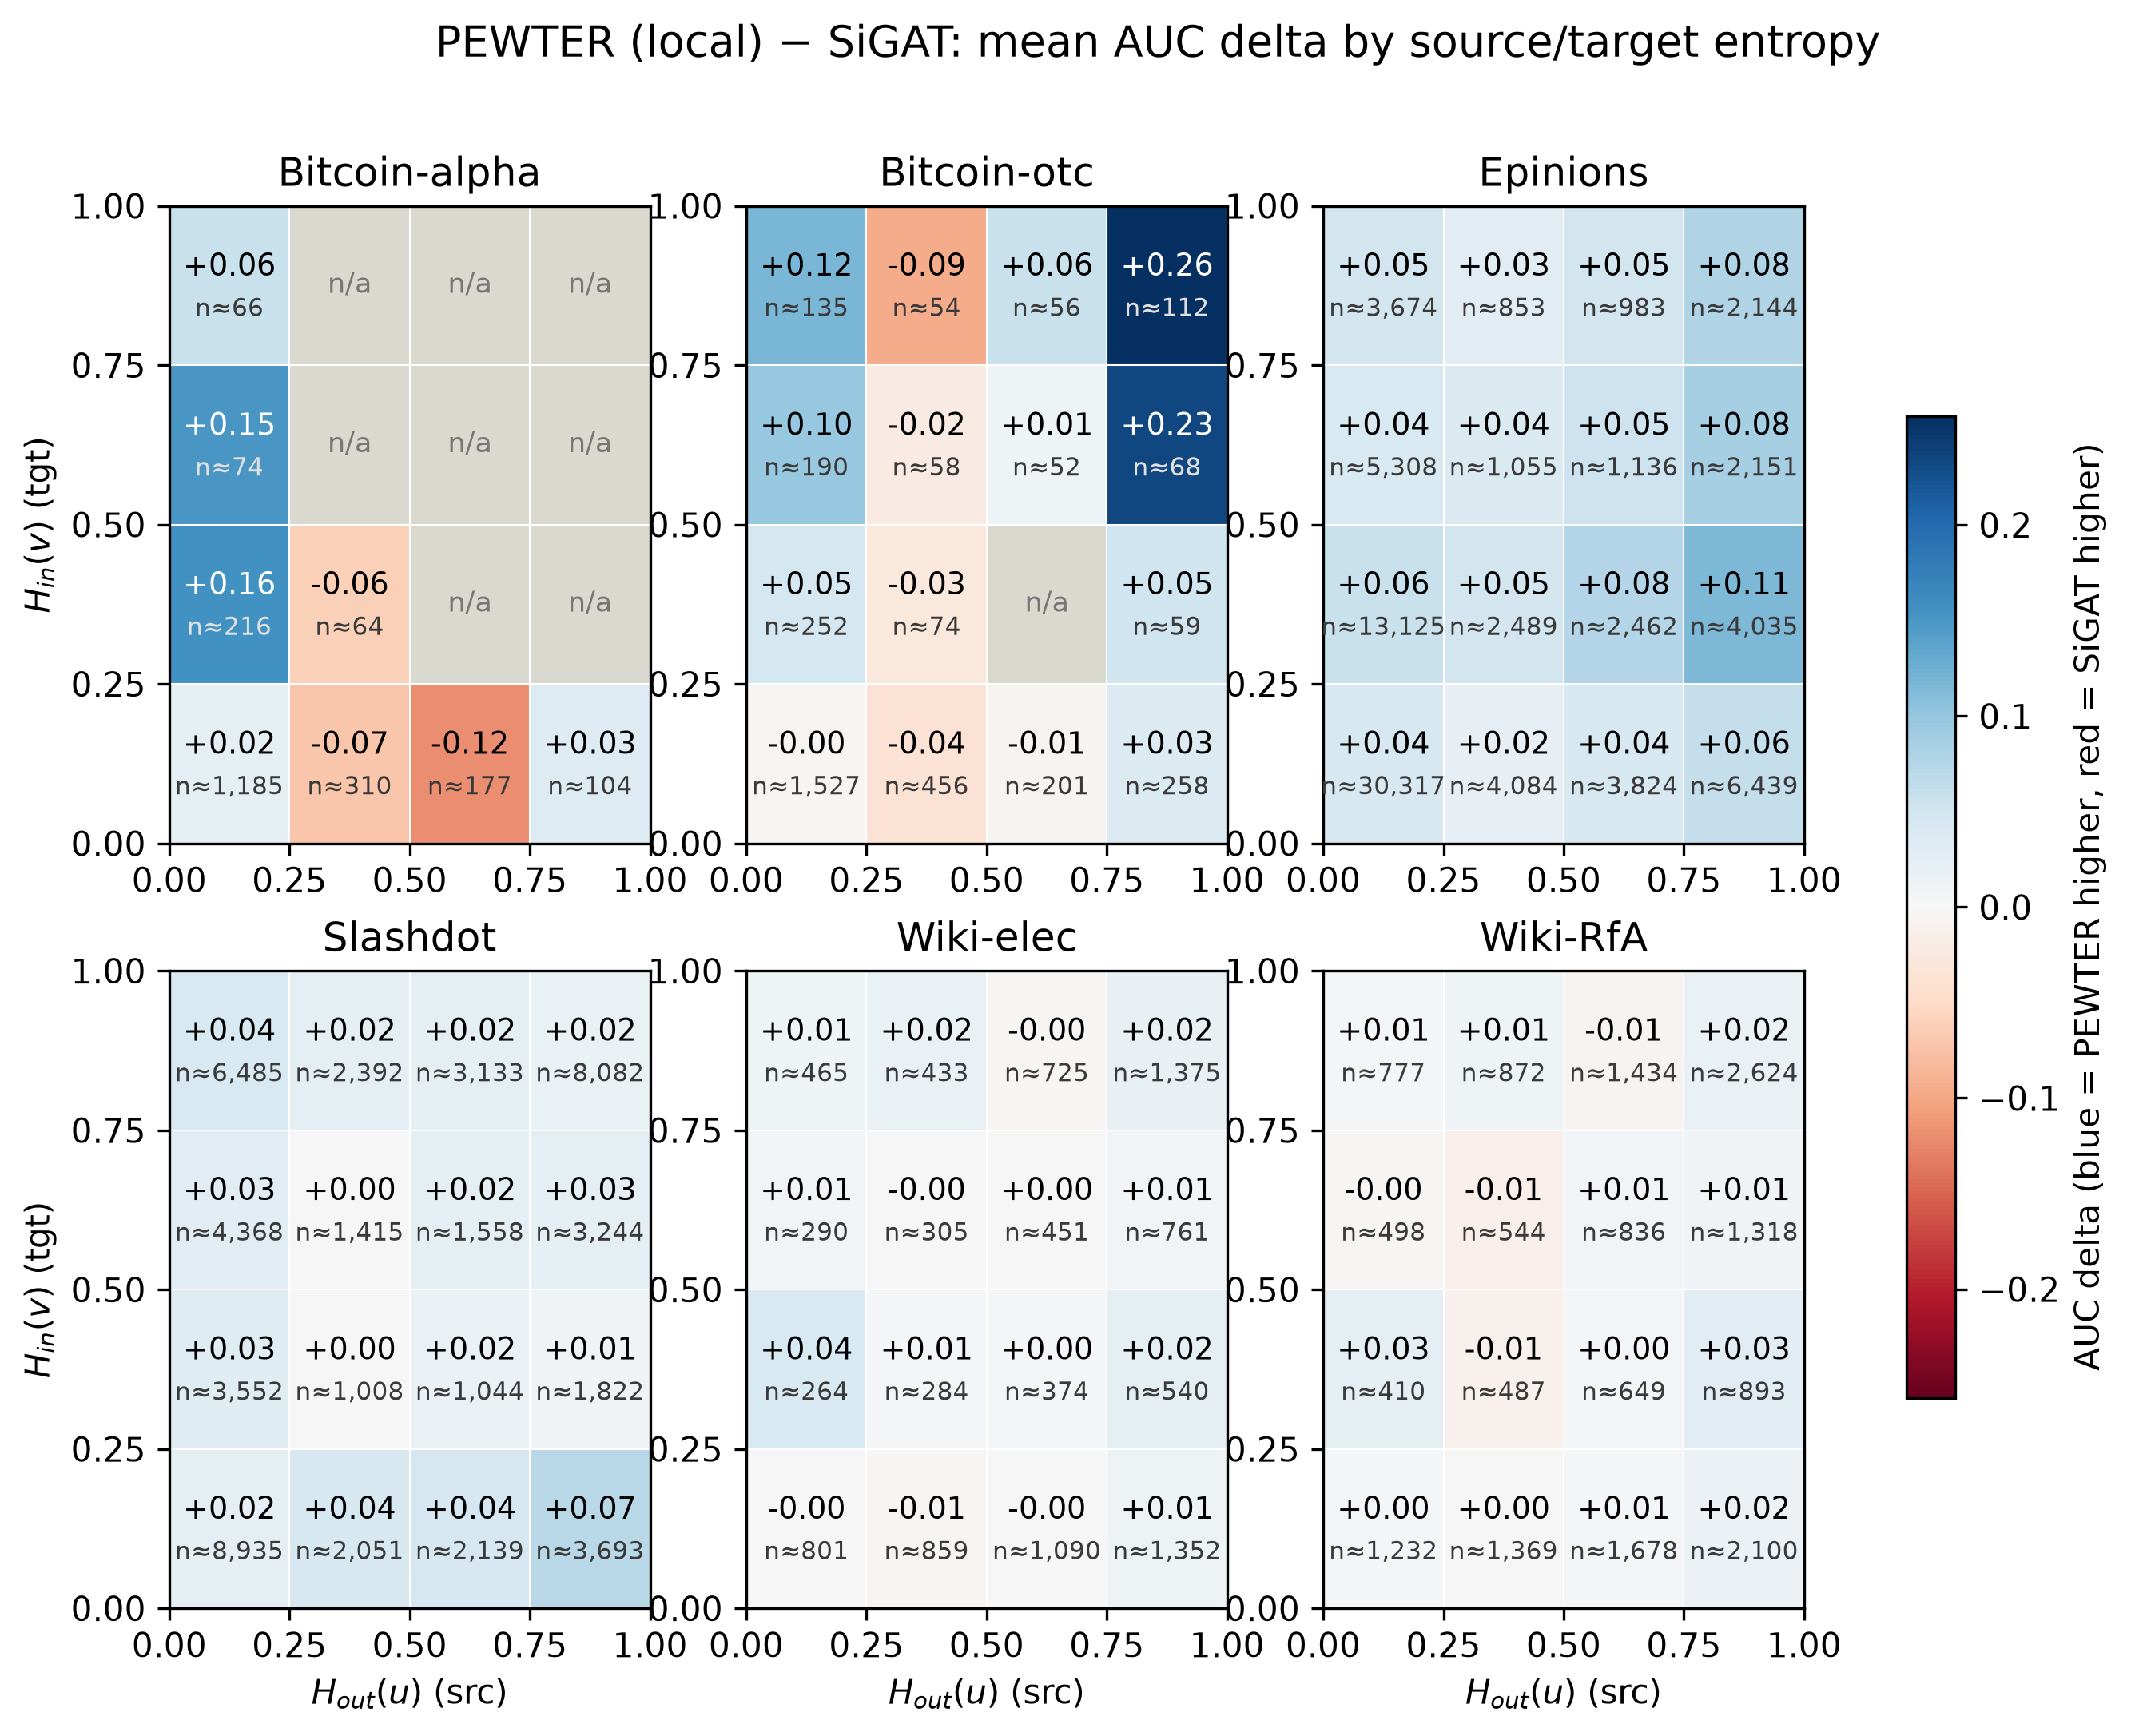
\includegraphics[width=\linewidth]{figures/pewter_sigat_delta_heatmap.png}
\caption{\method\ (local attention) minus SiGAT, mean test AUC by source/target entropy bin (10 splits, six datasets). Each cell shows the AUC delta and mean per-split sample size $n$ ($n\ge50$, else grey `n/a').}
\label{fig:delta-heatmap}
\end{figure}

\subsection{Relation between attention and entropy}

For every masked target-edge token we measure how attention mass at layer 0 splits between the source side ($u$, backward in the walk) and the target side ($v$, forward), and between vertex- and edge-token roles (Figure~\ref{fig:attndir}). This is a property of the trained attention weights, and a different question from the entropy asymmetry of Section~\ref{sec:empconf}(A): one describes what the data contains, the other where the model looks.

The split is heterogeneous, and significant on every dataset (cluster-robust 95\% CI on the forward-minus-backward difference excludes zero on all six, cluster = target edge; confirmed by a distribution-free Wilcoxon signed-rank test on the same per-edge cluster means). Two datasets are forward-dominant (Bitcoin-alpha $0.443$ forward vs.\ $0.411$ backward; Slashdot $0.417$ vs.\ $0.363$), and four are backward-dominant (Bitcoin-otc $0.403$ vs.\ $0.445$; Epinions $0.376$ vs.\ $0.452$; Wiki-elec $0.311$ vs.\ $0.432$; Wiki-RfA $0.189$ vs.\ $0.557$). We therefore do not claim that Pewter recovers a universal direction of information flow. What the measurement does show is that the model allocates attention asymmetrically at all, and that the asymmetry is dataset-specific rather than an artifact of the architecture, which is consistent with the heterogeneity found in the data itself. We checked whether this split tracks the source-minus-target entropy asymmetry of Section~\ref{sec:empconf}(C): the per-dataset forward-minus-backward attention mass and the per-dataset $\Hh_\outdeg-\Hh_\indeg$ gap correlate at Spearman $\rho=-0.71$ ($p=0.11$, $n=6$), a suggestive but not significant relationship at this sample size. We therefore keep this subsection as a descriptive observation rather than a claim that the two asymmetries are the same phenomenon.

Panel (D) asks the same directional question with a different instrument: instead of raw attention weight, we measure each context edge's exact Shapley contribution~\citep{shapley1953value} to the masked target's predicted sign probability (masking via the model's own \texttt{<MASK>} token, cluster-robust SE over target edges), decomposed by hop and direction within the $\pm2$-hop local window; "significant" here means the cluster-robust 95\% CI on the forward-minus-backward difference excludes zero. The two measurements do not always agree. Wiki-RfA's attention mass is the most backward-heavy of all six datasets ($0.189$ forward vs.\ $0.557$ backward), yet its hop-1 causal contribution is significantly \emph{forward}-dominant ($0.0098$ vs.\ $0.0070$); Wiki-elec and Slashdot also show a significant forward-dominant causal contribution, this time agreeing in direction with their attention split, while Bitcoin-alpha, Bitcoin-otc, and Epinions show no significant direction split by either measurement. Contribution also decays sharply from hop 1 to hop 2 on all six datasets in both directions, confirming that the $\pm2$-hop window is not spending its budget uniformly: the immediate neighbor edge does most of the causal work. The Wiki-RfA reversal is worth stating plainly: attention weight and causal contribution are not the same quantity, and a head can allocate more raw mass to backward tokens while those tokens' marginal effect on the actual prediction is smaller than the forward tokens'.

\begin{figure}[t!]
\centering
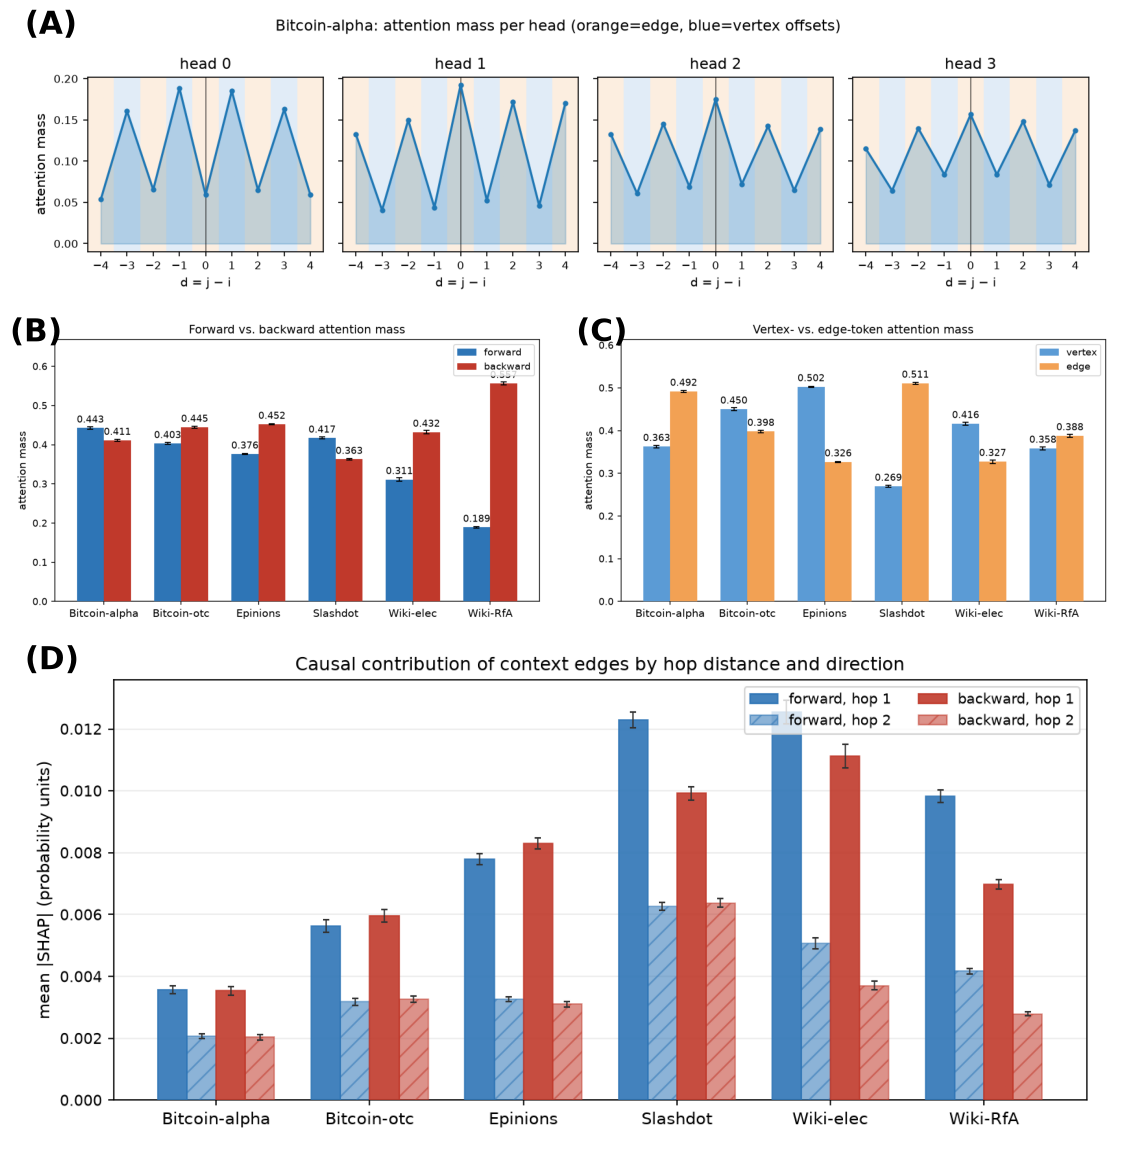
\includegraphics[width=\linewidth]{figures/attndir_panels_abcd_combined.png}
\caption{Attention directionality and causal contribution, \method, layer 0, six datasets. For each masked target-edge token $i$, attention mass is split by signed offset $d=j-i$ into forward ($d>0$, toward $v$'s side) and backward ($d<0$, toward $u$'s side), and by token role (vertex vs.\ edge); self-attention ($d=0$) is excluded. (A) Per-head breakdown (Bitcoin-alpha, 4 heads) over the window $d\in[-4,4]$: heads alternate their peak mass between vertex and edge offsets. (B) Forward vs.\ backward mass by dataset, mean over heads. (C) vertex vs.\ edge mass by dataset, mean over heads. (D) Causal contribution of context edges (exact Shapley value, not raw attention weight, on the masked target's predicted sign probability) by hop distance (1, 2 -- the full $\pm2$-hop window) and direction: contribution decays hop 1$\to$2 on all six datasets, both directions (cluster-robust SE, cluster = target edge); Wiki-elec, Wiki-RfA, and Slashdot are significantly forward-dominant at hop 1 (largest on Wiki-RfA), Bitcoin-alpha, Bitcoin-otc, and Epinions are not. Pewter here uses local attention throughout; this figure does not compare against the full-attention variant.}
\label{fig:attndir}
\end{figure}

\subsection{Ablations}

\paragraph{A) Proximal attention is sufficient.} Restricting attention to a $\pm2$-hop window matches or beats full attention on three of six datasets (Bitcoin-otc $+0.02$pp, Epinions $+0.13$pp, Wiki-elec $+0.15$pp) and trails on the other three (Bitcoin-alpha $-0.12$pp, Wiki-RfA $-0.09$pp, Slashdot $-0.21$pp); both variants appear in Table~\ref{tab:result1}. Every difference is within the reported standard errors, so the correct reading is that the local window costs nothing in accuracy rather than that it helps -- a genuine three-three split, not a lean toward either variant. A direct check finds that target edges have a labeled neighbor edge inside their attention window most of the time on all six datasets (Bitcoin-alpha $90.6\%$, Bitcoin-otc $89.2\%$, Epinions $84.6\%$, Slashdot $81.4\%$, Wiki-elec $74.9\%$, Wiki-RfA $87.9\%$), so the window captures real local context rather than an empty span; the lowest rate, on Wiki-elec, still leaves the window empty only when the walk itself runs out of visible context to offer.

\paragraph{B) The aggregator weighting is nearly irrelevant.} We compare the confidence weighting against 11 alternatives depending only on $q$, including the uniform mean, log-probability, certainty, Bernoulli-entropy and Fisher-information/inverse-variance forms (Table~\ref{tab:ablationB}, Appendix~\ref{app:extra}). Across all 11 functions on all 6 datasets the full spread is under $0.0018$ AUC -- an order of magnitude below the split-to-split std -- and the Fisher-information form is best on Epinions and Slashdot rather than our default. We report this as a null result: the gain of Pewter comes from the per-walk edge-centric representation, not from how the walks are pooled, and the aggregator should be treated as a design detail rather than as a contribution.

\paragraph{C) A single walk is already enough.} A given edge is scored by aggregating over hundreds to thousands of walk occurrences, raising a natural objection: is the reported gain just ensembling? We recompute test AUC as a function of $K$, the number of walk occurrences sampled per edge (uniform mean over $K$ occurrences drawn at random without replacement, mean $\pm$ std over the same 10 splits), sweeping $K=1,2,4,\ldots$ up to each dataset's own saturation point. AUC rises only slightly and quickly plateaus: the gap between $K=1$ and the saturated ceiling is under $1$pp on every dataset (Bitcoin-alpha $0.9085\to0.9133$, Bitcoin-otc $0.9278\to0.9317$, Epinions $0.9506\to0.9528$, Wiki-elec $0.8979\to0.9022$, Wiki-RfA $0.8874\to0.8914$, Slashdot $0.8883\to0.8967$), with saturation reached by $K\approx8$--$32$ on every dataset. More directly, a single walk with no aggregation at all already beats the best baseline on all six datasets (Table~\ref{tab:result1}). The representation, not the ensembling, carries the result; aggregating over more walk occurrences is a small, genuine, but secondary gain.

\subsection{Complexity}
Let $K$ be the number of corpus walks containing a given edge, an occurrence count that follows from the budget $M$ and length $L$ rather than a per-edge sampling parameter, and let $L$ be the maximum walk length in hops, so each walk is a token sequence of length at most $2L+1$. Sampling one walk costs $O(L)$; the per-walk transformer costs $O(L^2 d)$ under full attention and $O(Lwd)$ under the local window. Classifying one already-specified target edge therefore costs $O(K L^2 d)$, independent of $|V|$ and $|E|$ once $K$ and $L$ are fixed, unlike a $T$-layer message-passing GNN whose per-vertex receptive field, and hence per-edge inference cost, grows with local degree and $T$. The per-edge claim does not extend to the cost of covering a whole graph: the coverage guarantee requires a total budget $M=\kappa|E|$ for a small dataset-chosen constant $\kappa\in[1,5]$ (Setup below), so total sampling cost is $O(|E|)$ up to $\kappa$. Since $K$ is in the hundreds to thousands, the constant in front of the per-edge cost is much larger than a GNN's, and we report measured wall-clock cost alongside AUC rather than resting on the asymptotic statement \ph{TODO: add the wall-clock/throughput column or a small timing table. For a web-scale venue this is the single most likely reviewer objection to the method's practicality, and it is cheap to measure.} \ph{TODO: why $\kappa$ varies 1--5$\times$ by dataset (density? degree skew?) is not characterized, and no log-log wall-clock scaling curve across graph sizes has been measured; both are stated as future work in Section~\ref{sec:limits}.}

\section{Discussion and Limitations}
\label{sec:limits}
The bounds we prove concern what is conditioned on, so they apply to any vertex-centric read-out rather than to a particular architecture, and they are not removed by rewiring, depth, or width. Pewter sidesteps them by conditioning on labeled edges near the target, at the cost of sampling a walk corpus and running a transformer for every walk that contains a queried edge.

Several limitations bound what we can claim. The method assumes labeled edges near the target: on an edge whose neighborhood is entirely unlabeled, Pewter has nothing to condition on and degrades to the prior, whereas a vertex-centric model can still use a memorized endpoint embedding. Per-edge inference aggregates hundreds to thousands of walk evaluations, so the constant factor is high even though the asymptotic cost is independent of graph size. The two Wikipedia vote graphs behave differently from the four trust graphs on the directionality analysis, and we do not have a mechanism for that beyond the observation that a public vote and a private bilateral rating are different acts; six datasets from two genres is too few to settle it XXX MIGHT NOT BE TRUE WITH NEW RESULTS ON DIRECTIONALITY XXX. Finally, our bound is stated for the structural component of a model, and a fully transductive model with free per-vertex embeddings is outside its scope, as discussed after Assumption~\ref{as:structural}.

\section{Conclusion}
Reading an edge sign off two endpoint embeddings discards information in a way that is predictable from the label entropy that survives WL coarsening, and no depth or width recovers it. Pewter conditions instead on the labeled edges around the target, read directly from short walks, and pools across the walks that contain each edge. It improves AUC over eight baselines on six public signed networks, with the largest gains in the high-entropy regime the bound identifies (mean $+3.3$ AUC points over the best baseline per dataset, range $+1.4$ to $+4.5$). Two of our findings are negative and we think worth stating plainly: the direction of edge-sign information is not consistent across dataset genres, and how the per-walk predictions are pooled barely matters.

\section*{Ethical Considerations}
This work predicts trust and distrust signs on publicly available social and marketplace networks. We see four issues worth stating.

\emph{Data provenance and privacy.} All six datasets are public research benchmarks released by their original authors and widely used in prior work on signed networks; we collected no new data and interacted with no human subjects. vertices are pseudonymous identifiers, and we made no attempt to re-identify individuals, to link records across datasets, or to recover attributes beyond the graph structure and edge signs already present in the released files. The Wikipedia vote graphs derive from public deliberations whose participants had a reasonable expectation of visibility; the marketplace and review-site graphs derive from platform features whose users may not have anticipated research reuse, which is a limitation inherited from the benchmarks rather than introduced here.

\emph{Negative societal impact.} A model that predicts distrust edges predicts an accusatory statement about a named account. Deployed carelessly, such predictions could support automated reputation penalties, shadow-banning, or exclusion from a marketplace on the basis of an inferred rather than an actual judgement, and could be used to impute hostility between users who never expressed it. Predicted signs could also be used adversarially, for example to target users a model marks as likely to be distrusted, or to probe which of a user's ratings are inferable and therefore which are safe to withhold.

\emph{Distribution of errors.} All six datasets are heavily imbalanced toward positive edges (77--94\%), so a model tuned for aggregate AUC will make its errors disproportionately on the negative class, which is precisely the class with consequences for the person on the receiving end. Proposition~\ref{prop:bottleneck} implies a related fairness concern: error is forced upward exactly where endpoint label entropy is high, and contested or newly active accounts are over-represented there. Aggregate accuracy therefore understates the error rate faced by the users most likely to be affected by a decision.

\emph{Mitigations.} We recommend that predicted signs be used only as ranking or triage signals with a human decision-maker in the loop, never as an automatic basis for sanctioning an account; that any deployment report calibration and error rates separately for the negative class and for high-entropy endpoints rather than a single aggregate; and that predicted signs be labelled as inferred wherever they are surfaced, and not stored or displayed as if they were user-provided ratings. The models and datasets used here carry no dual-use capability beyond what the released benchmarks already permit, and we release code and configurations to make these error characteristics auditable rather than only the headline metric.

\begin{acks}
Anonymized funding acknowledgement and grants information.
\end{acks}

\appendix
\section{Full Proofs}
\label{app:proofs}
We work with a distribution $\mathcal{D}$ over labeled edges: draw an edge $(U,V)$ and read its label $Y$. All bounds are on the population (Bayes) error of the stated hypothesis class, which lower-bounds the test error of any member of that class.

\paragraph{Lemma (monotonicity and convexity of $\Hh_b^{-1}$).}
\emph{Monotonicity.} $\Hh_b$ restricted to $[0,\tfrac12]$ is a strictly increasing bijection onto $[0,1]$; write $f=\Hh_b|_{[0,\tfrac12]}$. Its inverse $f^{-1}=\Hh_b^{-1}$ is then strictly increasing: if $f^{-1}(x_1)\ge f^{-1}(x_2)$ for some $x_1<x_2$, applying the strictly increasing $f$ to both sides gives $x_1=f(f^{-1}(x_1))\ge f(f^{-1}(x_2))=x_2$, contradicting $x_1<x_2$. This licenses every ``larger entropy implies larger forced error'' reading in the main text and is used again below for the strict positivity in Proposition~\ref{prop:bottleneck} and the substitution in Proposition~\ref{prop:capacity}.

\emph{Convexity.} $f$ is strictly concave. The inverse of a strictly increasing, strictly concave function is strictly convex: for $x,y\in[0,\tfrac12]$ and $\alpha,\beta>0$ with $\alpha+\beta=1$, strict concavity gives $f(\alpha x+\beta y) > \alpha f(x)+\beta f(y)$. Since $f^{-1}$ is strictly increasing, applying it to both sides preserves the inequality; writing $X=f(x)$, $Y=f(y)$,
\[
\alpha f^{-1}(X)+\beta f^{-1}(Y) \ =\ \alpha x+\beta y \ >\ f^{-1}(\alpha X+\beta Y),
\]
which is strict convexity of $\Hh_b^{-1}$ on $[0,1]$. Neither argument needs differentiability. Convexity licenses the Jensen step below.

\paragraph{Pinsker-type relaxation.} XXX REF TO PINSKER XXX $\Hh_b^{-1}$ has no elementary closed form. The bound $\Hh_b(p)\le 1-\tfrac{2}{\ln 2}(\tfrac12-p)^2$~\citep{cover2006elements} gives the explicit, slightly looser alternative
\begin{equation}
P_e\ \ge\ \tfrac12-\sqrt{\tfrac{\ln 2}{2}\big(1-\Hh(Y\mid Z)\big)},
\label{eq:pinsker}
\end{equation}
which may be substituted for \eqref{eq:invfano} wherever an explicit formula is preferred.

\paragraph{Proposition~\ref{prop:bottleneck}.}
\emph{Setup.} A message-passing GNN with any finite number $T$ of rounds assigns to each vertex a color $\chi_T(\cdot)$ that refines to at most the stable WL coloring, and the vertex representation is a fixed function of that color, $h_u=\psi(\chi_T(u))$~\citep{xu2018powerful,morris2019weisfeiler}. Hence any edge read-out satisfies $\hat y_{uv}=g(\psi(\chi_T(u)),\psi(\chi_T(v)))=\tilde g(\chi_T(u),\chi_T(v))$, so $\hat Y$ is measurable with respect to the $\sigma$-algebra $\mathcal{F}$ generated by the color pair $(\chi_T(U),\chi_T(V))$.

\emph{Bound.} Among all $\mathcal{F}$-measurable predictors the error is minimized by the maximum-a-posteriori rule $\tilde g^\star(a,b)=\arg\max_y \Pr(Y=y\mid \chi_T(U)=a,\chi_T(V)=b)$. Conditional on a fixed color pair $(a,b)$ this is the binary problem of the Problem Setting, so $P_e(a,b)\ge \Hh_b^{-1}\big(\Hh(Y\mid \chi_T(U)=a,\chi_T(V)=b)\big)$. The overall error is $P_e=\mathbb{E}_{(a,b)}[P_e(a,b)]$; applying Jensen's inequality to the convex $\Hh_b^{-1}$ gives
\begin{multline*}
P_e \ \ge\ \mathbb{E}_{(a,b)}\Big[\Hh_b^{-1}\big(\Hh(Y\mid a,b)\big)\Big] \ \ge\ \Hh_b^{-1}\Big(\mathbb{E}_{(a,b)}\big[\Hh(Y\mid a,b)\big]\Big) \\
\ =\ \Hh_b^{-1}\big(\Hh(Y\mid \chi_T(U),\chi_T(V))\big),
\end{multline*}
the last step being the chain rule for conditional entropy. Since any GNN lies in this class, its error is at least this bound. Because $\chi_T$ refines toward the stable coloring $\chi$, $\Hh(Y\mid \chi_T(U),\chi_T(V))\ge \Hh(Y\mid \chi(U),\chi(V))$, and $\Hh_b^{-1}$ is increasing, so the bound at the stable coloring lower-bounds the bound at any finite $T$. Assumption~\ref{as:structural} makes $\Hh(Y\mid \chi(U),\chi(V))$ strictly positive, hence $P_e>0$. Neither depth nor width lowers it, since both only refine within the WL ceiling.

\emph{Identity versus color.} In a simple graph the identity pair $(U,V)$ fixes the unique incident edge, so $\Hh(Y\mid U,V)=0$; the whole bound is the information gap $\Hh(Y\mid \chi(U),\chi(V))-\Hh(Y\mid U,V)$ destroyed by replacing identities with colors. This is why the multiplicity of edges per pair is irrelevant to the argument.

\emph{Corollary~\ref{cor:endpoint}.} Fix a source $u$ and a target color $b$. All edges from $u$ to color-$b$ targets share the color pair $(\chi(u),b)$ and receive one prediction, so by \eqref{eq:invfano} applied to this single color pair, with no averaging and hence no Jensen step, their error is at least $\Hh_b^{-1}\big(\Hh(Y\mid \text{source}{=}u,\text{target color}{=}b)\big)$. If $u$'s out-edges carry mixed labels not separated by target color, this entropy is close to $\Hh_\outdeg(u)$, recovering the single-endpoint reading. $\square$

\paragraph{Proposition~\ref{prop:capacity}.}
Let each embedding take at most $N$ distinguishable values under the read-out. A variable supported on $\le N$ values has entropy $\le \log N$, so $\MI(Y;h_U,h_V)\le \Hh(h_U,h_V)\le \Hh(h_U)+\Hh(h_V)\le 2\log N$. Substituting into $\Hh(Y\mid h_U,h_V)=\Hh(Y)-\MI(Y;h_U,h_V)$ gives $\Hh(Y\mid h_U,h_V)\ge \Hh(Y)-2\log N$. Applying \eqref{eq:invfano} and using that $\Hh_b^{-1}$ is increasing, $P_e\ge \Hh_b^{-1}\big(\Hh(Y)-2\log N\big)$; with the convention $\Hh_b^{-1}(x):=0$ for $x\le0$ this is unconditionally true, but informative only when $\Hh(Y)>2\log N$. For the per-vertex statement, $h_U$ alone satisfies $\MI(\{Y_e\}_{e\ni U}; h_U)\le \Hh(h_U)\le \log N$, while $D$ near-independent out-edge labels of entropy $\Hh_\outdeg(U)$ each carry $D\,\Hh_\outdeg(U)$ bits; once this exceeds $\log N$ the excess cannot pass through the shared embedding. $\square$

\paragraph{General $c$.} For $c>2$ the exact binary specialization does not apply directly. Weakening \eqref{eq:fano} using $\Hh_b(P_e)\le 1$ and $\log(c-1)\le\log c$ gives the linear corollary
\[
P_e\ \ge\ \frac{\Hh(Y\mid Z)-1}{\log c},
\]
valid and non-vacuous for $c>2$, unlike at $c=2$. Proposition~\ref{prop:bottleneck}, Corollary~\ref{cor:endpoint} and Proposition~\ref{prop:capacity} all hold in this form by the same arguments, replacing every $\Hh_b^{-1}(\cdot)$ with $(\cdot-1)/\log c$; the averaging step in Proposition~\ref{prop:bottleneck} needs no Jensen argument here, since an affine function is both convex and concave.

\label{app:extra}

\begin{table}[h!]
\centering
\scriptsize
\caption{Ablation B: test AUC (mean $\pm$ std, 10 splits) for Pewter (local attention) under 11 aggregator weight functions $w(q)$, each depending only on the walk's predicted probability $q$. Bold marks the best per dataset, italic the second best. The full spread across all functions and datasets is under $0.0018$ AUC -- an order of magnitude below the split-to-split std -- confirming the aggregator choice is noise-level, not a real effect.}
\label{tab:ablationB}
\resizebox{\linewidth}{!}{%
\begin{tabular}{lcccccc}
\toprule
Weight $w(q)$ & Bitcoin-alpha & Bitcoin-otc & Epinions & Wiki-elec & Wiki-RfA & Slashdot \\
\midrule
Uniform (mean) & $0.913_{\pm0.017}$ & $0.932_{\pm0.006}$ & $0.953_{\pm0.001}$ & $0.902_{\pm0.003}$ & $0.891_{\pm0.005}$ & $0.897_{\pm0.002}$ \\
$q^b$ & $\mathbf{0.914_{\pm0.017}}$ & $0.932_{\pm0.007}$ & $0.953_{\pm0.001}$ & $\mathbf{0.902_{\pm0.003}}$ & $0.891_{\pm0.005}$ & $0.897_{\pm0.002}$ \\
$\exp(bq)$ & $0.913_{\pm0.018}$ & $\mathbf{0.932_{\pm0.007}}$ & $0.953_{\pm0.001}$ & $0.902_{\pm0.003}$ & $0.891_{\pm0.005}$ & $0.897_{\pm0.002}$ \\
$|q-0.5|^b$ & $0.913_{\pm0.017}$ & $\mathit{0.932_{\pm0.007}}$ & $0.953_{\pm0.002}$ & $0.902_{\pm0.003}$ & $0.891_{\pm0.005}$ & $0.897_{\pm0.002}$ \\
$\mathrm{sig}(b(q-0.5))$ & $\mathit{0.914_{\pm0.017}}$ & $0.932_{\pm0.007}$ & $0.953_{\pm0.001}$ & $0.902_{\pm0.003}$ & $0.891_{\pm0.005}$ & $0.897_{\pm0.002}$ \\
$(-\log q)^b$ & $0.912_{\pm0.017}$ & $0.932_{\pm0.007}$ & $0.953_{\pm0.001}$ & $0.902_{\pm0.003}$ & $0.891_{\pm0.005}$ & $0.897_{\pm0.002}$ \\
$|\mathrm{logit}(q)|^b$ (default) & $0.913_{\pm0.017}$ & $0.932_{\pm0.007}$ & $0.954_{\pm0.002}$ & $0.902_{\pm0.003}$ & $0.891_{\pm0.005}$ & $0.897_{\pm0.002}$ \\
$(\ln2-H(q))^b$ & $0.913_{\pm0.017}$ & $0.932_{\pm0.007}$ & $0.953_{\pm0.002}$ & $0.902_{\pm0.003}$ & $0.891_{\pm0.005}$ & $0.897_{\pm0.002}$ \\
$\exp(-aH(q))$ & $0.913_{\pm0.017}$ & $0.932_{\pm0.006}$ & $\mathit{0.954_{\pm0.002}}$ & $0.902_{\pm0.003}$ & $\mathbf{0.891_{\pm0.005}}$ & $\mathit{0.897_{\pm0.002}}$ \\
$(q(1-q))^{-b}$ (Fisher-info) & $0.913_{\pm0.017}$ & $0.932_{\pm0.007}$ & $\mathbf{0.954_{\pm0.002}}$ & $\mathit{0.902_{\pm0.003}}$ & $\mathit{0.891_{\pm0.005}}$ & $\mathbf{0.897_{\pm0.002}}$ \\
$\max(q,1-q)^b$ & $0.913_{\pm0.017}$ & $0.932_{\pm0.006}$ & $0.953_{\pm0.002}$ & $0.902_{\pm0.003}$ & $0.891_{\pm0.005}$ & $0.897_{\pm0.002}$ \\
\bottomrule
\end{tabular}%
}
\end{table}
%% References Section
\bibliographystyle{ACM-Reference-Format}
\bibliography{pewter_references}

\end{document}
